\newpage
\subsection{IT-Asset-Management (ITAM)}
Grundlage des IT-Risikomanagements ist ein IT-Asset-Management: ein System, in dem die gesamte eingesetzte Hardware und ggf. auch Software und Lizenzen erfasst werden, beispielsweise:
\begin{itemize}
  \item Serverhardware
  \item Virtuelle Maschinen oder Container bei externen Dienstleistern
  \item Netzwerkhardware wie Switches, Router, Firewalls etc.
  \item Hardware in Büros wie WLAN-Access-Points, DHCP-Server, Drucker etc.
  \item IoT-Geräte
  \item OT-Systeme (Operational Technology)
  \item Sicherheitshardware wie Kameras, Zugangssysteme etc.
  \item Desktop-PCs, Notebooks und mobile Endgeräte wie Smartphones oder Tablets
\end{itemize}

Das Unternehmen muss definieren und dokumentieren, was ein Asset ist und ab wann es erfasst werden muss. Der Begriff kann weiter gefasst werden und Personen, Informationen oder Prozesse einschließen, etwa Geschäftsgeheimnisse, die im Risikomanagement als besonders schützenswert gelten. Grundsätzlich sollte jede betriebsrelevante Hardware erfasst werden, auch Testsysteme, da diese ebenfalls betriebskritisch sein können. Ob Server, VMs oder Container im eigenen Serverraum oder im Managed-Hosting-Rechenzentrum laufen, spielt keine Rolle. NIS2 macht keine Vorgaben zur Ausgestaltung; theoretisch genügt eine strukturierte Excel-Liste. Es gibt jedoch spezialisierte Open-Source-Lösungen wie Snipe-IT, NetBox, Ralph oder GLPI.

Neben Betriebssystem, Software und genauer Modellbezeichnung sollten, sofern verfügbar, das End-of-Life-Datum und ein verantwortlicher Asset-Owner dokumentiert werden; das hilft später u.\,a. beim Lebenszyklus- und Schwachstellenmanagement. Die Herausforderung liegt nicht nur in der initialen Erfassung, sondern im aktuellen Halten des Inventars in einer dynamischen IT-Umgebung. Je nach Infrastruktur helfen automatisierte Scanner oder Skripte, die das Netzwerk nach neuen Geräten durchsuchen, sowie Agenten, die installierte Hard- und Software erfassen und melden.
\newpage
Besonders komplex ist die Asset-Verwaltung in Cloud-Umgebungen, da Ressourcen dynamisch erstellt und gelöscht werden. Infrastructure-as-Code-Ansätze schaffen hier programmatische Sichtbarkeit; über Cloud-Provider-APIs lassen sich auch kurzlebige Ressourcen wie Container oder serverlose Funktionen erfassen.

Die Nutzung des Asset-Management-Systems muss nachvollziehbar dokumentiert sein, inklusive eines eindeutigen Prozesses für die Erfassung und die Entfernung bei Ausmusterung. Ein Prozessverantwortlicher sollte die Einhaltung kontrollieren, den Prozess verbessern und als zentraler Ansprechpartner dienen.

Für Datenträger und Geräte mit sensiblen Informationen muss ein Prozess zur sicheren Löschung bzw. Entsorgung definiert werden, idealerweise als verbindliche, im Unternehmen kommunizierte Arbeitsanweisung.

Eine weitere Herausforderung ist Schatten-IT: Geräte oder Software, die ohne Genehmigung und Wissen der IT-Abteilung genutzt und daher nicht überwacht und verwaltet werden. Neben einer Richtlinie zur Nutzung privater Hardware (BYOD, Bring Your Own Device) sollte die IT weitere Maßnahmen ergreifen, etwa automatische Netzwerkscans nach unbekannten Geräten bzw. MAC-Adressen.
\newpage
\textbf{Checkliste: Asset-Management}
\begin{checklist}
  \item Festlegen, was in der Organisation als Asset gilt (z.\,B. IT-Systeme, Software, Daten, Services)
  \item Definieren, welche Informationen zu einem Asset erfasst werden müssen (z.\,B. Name, Standort, Owner, Zweck, Hardware-Typ, Betriebssystem, Schnittstellen)
  \item Festlegen eines fachlichen Asset Owners mit klarer Verantwortung
  \item Klassifizieren der Assets nach Kritikalität und Schutzbedarf (Verfügbarkeit, Integrität, Vertraulichkeit)
  \item Auswahl eines geeigneten Tools zur zentralen Erfassung und Pflege der Assets
  \item Definieren eines Prozesses zur Identifikation und initialen Erfassung neuer Assets
  \item Definieren eines Prozesses zur Pflege und Aktualisierung von Asset-Informationen bei Änderungen
  \item Definieren eines Prozesses zur Außerbetriebnahme und Entsorgung von Assets
  \item Definieren eines Prozesses zur sicheren Vernichtung von Datenträgern oder Geräten mit sensiblen Informationen
  \item Regelmäßiger Abgleich zwischen dokumentiertem Asset-Bestand und tatsächlicher Umgebung (Dokumentation vs. Realität)
\end{checklist}
\newpage
\subsection{IT-Risikomanagement}
Das IT-Risikomanagement ist ein zentraler Punkt von NIS2. Ziel ist es, die Infrastruktur hinsichtlich potenzieller Risiken zu bewerten und diesen mit technischen oder organisatorischen Maßnahmen zu begegnen. Ergebnis ist also nicht nur die Risikoanalyse selbst, sondern auch die daraus abgeleiteten Maßnahmen.

Zunächst muss die Organisation den Begriff Risiko für sich definieren. Typischerweise sind Risiken Ereignisse, die bei Eintritt die Informationssicherheitsziele (Vertraulichkeit, Verfügbarkeit, Integrität) oder Geschäftsziele beeinträchtigen. Vor der Risikoanalyse sollten zudem folgende Begriffe bestimmt werden:

Das \textbf{Gesamtrisikoprofil} fasst alle relevanten Risiken der Organisation verdichtet zusammen und beantwortet die Frage: Wie riskant ist unser Unternehmen insgesamt? Neben IT-Risiken fließen operationelle, finanzielle und strategische Risiken ein. Ein vollständiges Bild entsteht erst mit ESG-Risiken (Environmental, Social, Governance), die zunehmend regulatorische Bedeutung gewinnen.

\textbf{Risikotoleranz} beschreibt, wie viel Risiko eine Organisation bewusst eingehen will, um ihre strategischen Ziele zu erreichen.

\textbf{Inhärentes Risiko} und \textbf{Residualrisiko}: Das inhärente Risiko (Bruttorisiko) ist das Risiko vor jeglichen Gegenmaßnahmen, das Residualrisiko (Restrisiko) das nach Umsetzung aller Maßnahmen verbleibende Risiko. Ihre Differenz zeigt, wie wirksam die Kontrollen sind. Geschäftsleitungen müssen verstehen, dass Risiken nie auf null sinken und sie das Restrisiko formal akzeptieren müssen.

Das \textbf{Risikodeckungspotenzial} beschreibt, wie viel Risiko eine Organisation finanziell und organisatorisch abfedern kann, ohne in existenzielle Schwierigkeiten zu geraten, typischerweise durch Eigenkapital, liquide Reserven und Versicherungen. Die \textbf{Risikotragfähigkeit} setzt das Gesamtrisikoprofil ins Verhältnis zum Deckungspotenzial: Liegt unser Gesamtrisiko innerhalb dessen, was wir verkraften können? Wenn nicht, besteht akuter Handlungsbedarf.
\newpage
Zusätzlich empfiehlt es sich, Risikoklassen anhand des Risikodeckungspotenzials zu definieren. Die niedrigste Klasse umfasst Risiken mit vernachlässigbaren Auswirkungen. Ein Beispiel:

\tcbset{colback=gray!5!white, colframe=gray!70!black, boxrule=0.3mm, arc=1mm, left=1mm, right=1mm, top=0.5mm, bottom=0.5mm}

\begin{tcolorbox}[title=Klasse 1: Minimal]
Kaum Auswirkungen, Verluste unter 1.000\texteuro. Risiko akzeptabel, keine Maßnahmen.
\end{tcolorbox}

\begin{tcolorbox}[title=Klasse 2: Niedrig]
Geringfügige Beeinträchtigungen, Verluste 1.000–10.000\texteuro. Überwachung empfohlen.
\end{tcolorbox}

\begin{tcolorbox}[title=Klasse 3: Mittel]
Spürbare Auswirkungen, Verluste 10.000–100.000\texteuro. Maßnahmen erforderlich.
\end{tcolorbox}

\begin{tcolorbox}[title=Klasse 4: Hoch]
Erhebliche Störung, Verluste 100.000–1.000.000\texteuro. Sofortiges Eingreifen notwendig.
\end{tcolorbox}

\begin{tcolorbox}[title=Klasse 5: Kritisch]
Existenzbedrohend, Verluste $>\,$1.000.000\texteuro. Notfallmaßnahmen zwingend.
\end{tcolorbox}

Klassen, Definitionen und Werte dienen nur als Orientierung und können je nach Organisation angepasst werden.

Als Nächstes ist ein IT-Risikomanagement-Modell auszuwählen und die Entscheidung begründet zu dokumentieren. Verbreitete Frameworks sind ISO 27005, NIST RMF, COSO ERM und BSI 200-3. Sie haben alle ihre Berechtigung, sind aber komplex und für kleinere Unternehmen möglicherweise zu umfangreich. NIS2 verlangt nur angemessene Maßnahmen. Ist das Unternehmen zu klein, fehlen personelle Kapazitäten oder sind die Prozesse der Frameworks zu starr, ist ein eigenes Risikomanagement legitim. Auch dies ist in der Dokumentation zu begründen. Wichtig ist, dass der Prozess für alle IT-Systeme identisch abläuft. Er darf (und muss ggf.) punktuell angepasst werden, aber nicht ohne Grund, da sonst Vergleichbarkeit und Kontinuität leiden. Jedes IT-Risikomanagement umfasst mindestens vier Phasen: Risiken identifizieren, Risiken bewerten, Risiken behandeln und Monitoring.

Der Prozess muss regelmäßig wiederholt werden, um zu prüfen, ob Maßnahmen noch aktuell sind oder neue Risiken entstanden sind, und sollte kontinuierlich verbessert werden. Ebenso ist er durchzuführen, wenn Komponenten hinzugefügt oder ausgetauscht werden.
\newpage
\subsubsection{Phase 1: Risiken identifizieren}
In der ersten Phase sollen potenzielle Risiken möglichst vollständig identifiziert werden, unabhängig von Eintrittswahrscheinlichkeit oder Schwere. Ziel ist nicht die Bewertung oder Priorisierung, sondern alle relevanten Risikoszenarien sichtbar zu machen.

Im Fokus stehen Risiken für Verfügbarkeit, Integrität und Vertraulichkeit von Informationen, IT-Systemen und unterstützenden Prozessen. Ausgangspunkt ist in der Regel das IT-Asset-Management: Für jedes Asset wird betrachtet, welchen Bedrohungen und Schwachstellen es ausgesetzt sein könnte. Ähnliche Systeme können zusammengefasst werden. So besteht bei nahezu jeder Hardware das Risiko eines Ausfalls von Festplatten, Netzteilen oder anderen Komponenten. Auch Systeme gleicher Funktion, etwa Datenbank- oder Webserver, lassen sich gruppieren, um die Übersicht zu wahren.

Die Identifikation sollte strukturiert, aber bewusst offen gestaltet werden. Bewährt hat sich ein gemeinsames Brainstorming mehrerer Mitarbeitender mit Kenntnis der IT-Umgebung und Geschäftsprozesse. Alternativ sammeln zunächst kleine Gruppen eigene Risikoszenarien, die anschließend zusammengeführt, diskutiert und ergänzt werden. Methoden wie Brainwriting oder die 6-3-5-Methode helfen, auch weniger offensichtliche Risiken sichtbar zu machen.

Neben technischen sind auch organisatorische, personelle und externe Risiken zu berücksichtigen, etwa Abhängigkeiten von Dienstleistern, Ausfall von Schlüsselpersonal oder eine veränderte Bedrohungslage. Wer wenig Erfahrung hat, kann sich an Rahmenwerken orientieren, etwa am BSI-Standard 200-3, der ein schlankes Risikomanagement-Framework sowie eine Liste von Gefährdungskategorien bereitstellt.
\newpage
\subsubsection{Phase 2: Risiken bewerten}
Anschließend werden die Risiken bewertet, um Relevanz und Priorität einzuschätzen. Die wichtigsten Kriterien sind \textbf{Eintrittswahrscheinlichkeit} und \textbf{Schadauswirkung}. Denkbar sind weitere Faktoren wie Erkennbarkeit, Kontrollierbarkeit, Kaskadeneffekte, Wiederherstellungszeit oder die Zeit bis zum Schadenseintritt.

Für ein praktikables Risikomanagement genügt es zunächst, sich auf Eintrittswahrscheinlichkeit und Schadauswirkung zu konzentrieren. Weitere Faktoren können bei besonders kritischen oder komplexen Risiken ergänzt werden.

Bewertet wird üblicherweise auf einer numerischen Skala (z.\,B. 1 bis 5), deren Werte klar beschrieben sein müssen, um eine einheitliche Bewertung zu ermöglichen. Die Bewertung ist kein rein technischer Vorgang, sondern ein Abstimmungsprozess mit verschiedenen Personen und Fachbereichen, sodass unterschiedliche Perspektiven einfließen.

Objektive Messwerte gibt es selten; Einschätzungen beruhen oft auf Erfahrung, Annahmen und fachlichem Urteil. Um diese Subjektivität zu reduzieren, sollten Risiken gemeinsam diskutiert und Bewertungen nachvollziehbar begründet werden, mit dem Ziel einer konsistenten Einschätzung.

Aus beiden Faktoren ergibt sich der Risikowert: $Schadauswirkung \times Eintrittswahrscheinlichkeit$. Er dient als vereinfachte Kennzahl zur Priorisierung: Je höher der Wert, desto kritischer das Risiko und desto dringlicher die Behandlung.
\newpage
\begin{figure}[htbp]
  \centering
  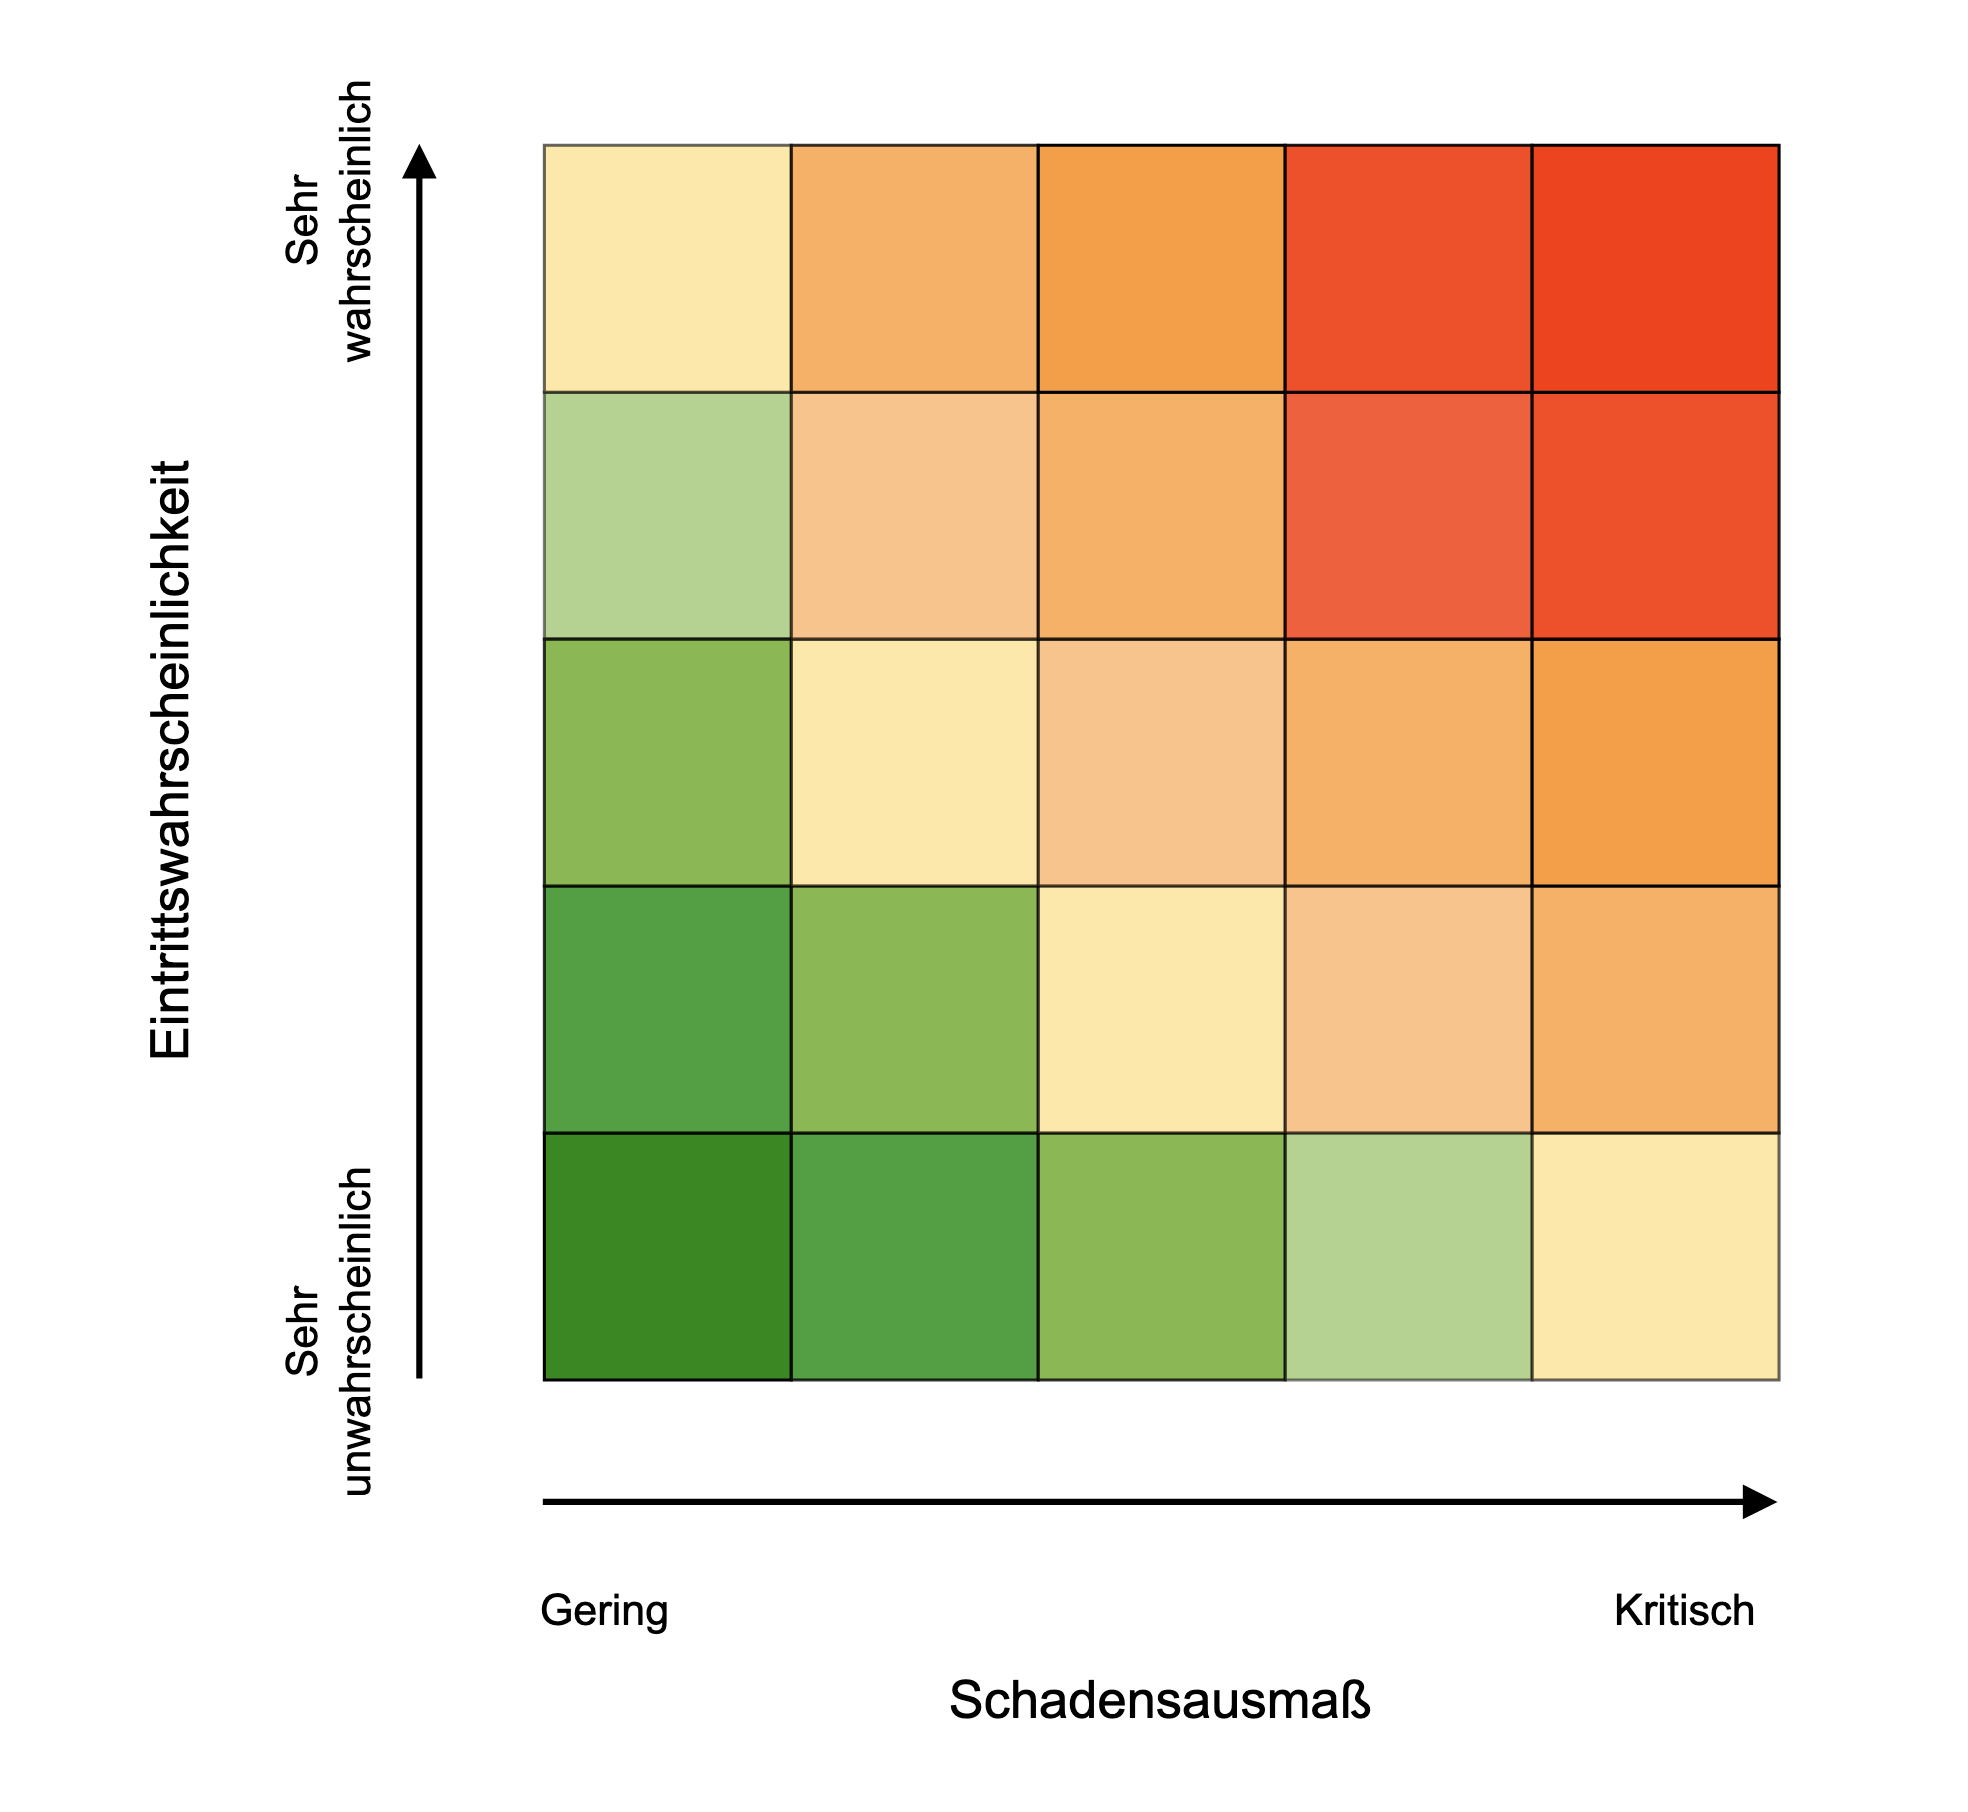
\includegraphics[width=0.55\textwidth]{images/Risikomatrix.png}
  \caption{Beispiel einer Risikomatrix}
  \label{fig:risikomatrix}
\end{figure}

Zur Übersicht können die bewerteten Risiken in einer Risikomatrix mit Schadauswirkung und Eintrittswahrscheinlichkeit als Achsen dargestellt werden, sodass kritische Risiken auf einen Blick erkennbar sind.



\newpage
\subsubsection{Phase 3: Maßnahmen ergreifen}

Risiken werden nach Priorität behandelt, hoch bewertete zuerst. Grundsätzlich gibt es vier Behandlungsoptionen:
\begin{itemize}
  \item \textbf{Vermeiden}: Das Risiko wird vermieden, indem die zugrunde liegende Tätigkeit nicht durchgeführt oder ein IT-System nicht betrieben bzw. abgeschaltet wird.
  \item \textbf{Mindern}: Durch technische oder organisatorische Maßnahmen wird die Eintrittswahrscheinlichkeit oder die Schadauswirkung eines Risikos reduziert.
  \item \textbf{Transferieren}: Das Risiko wird ganz oder teilweise an Dritte übertragen, beispielsweise durch Outsourcing oder den Abschluss von Versicherungen.
  \item \textbf{Akzeptieren}: Das Risiko wird bewusst akzeptiert, da es als tragbar eingeschätzt wird.
\end{itemize}

Die Wahl hängt von den Gegebenheiten der Organisation ab. In der Praxis werden Risiken meist gemindert, etwa durch Zwei-Faktor-Authentifizierung gegen die unbefugte Übernahme von Benutzerkonten. Welche Maßnahmen geeignet sind, hängt u.\,a. von Kosten, Nutzen und Umsetzungsaufwand ab. Fachabteilungen oder IT-Teams können Maßnahmen vorschlagen; über Priorisierung und Ressourceneinsatz entscheidet in der Regel das Management.

Beim Transfer durch Outsourcing oder Versicherungen verschwindet das Risiko nicht: Es entstehen neue Abhängigkeiten, und die Verantwortung für Auswahl, Steuerung und Überwachung der Dienstleister bleibt bestehen.

Das Vermeiden durch Unterlassen einer Aktivität oder Abschalten eines Systems kommt vor allem bei neuen Vorhaben oder nicht geschäftskritischen Systemen in Betracht, da es bei bestehenden Infrastrukturen oft nur eingeschränkt möglich ist.

Akzeptiert werden vor allem Risiken mit geringer Auswirkung oder solche, die als tragbar gelten. Akzeptieren heißt nicht ignorieren: Die Organisation kennt durch die Analyse Eintrittswahrscheinlichkeit und möglichen Schaden und entscheidet sich bewusst gegen weitere Maßnahmen.

Unabhängig von der Strategie verbleibt meist ein Restrisiko. Behandlungsentscheidung und akzeptiertes Restrisiko sind mit kurzer Begründung zu dokumentieren; das erhöht die Nachvollziehbarkeit bei Audits und erneuten Risikoanalysen.
\newpage
Manche Risiken sollten im Business Continuity Management (BCM) behandelt werden: solche, die kritische Geschäftsprozesse bedrohen (ob technisch oder organisatorisch) und deren Unterbrechungseffekte definierte Toleranzen überschreiten, insbesondere wenn ihre Auswirkungen das Risikodeckungspotenzial bzw. die Risikotragfähigkeit übersteigen. Sie lassen sich nicht allein durch Prävention oder Kontrollen beherrschen, sondern erfordern vorbereitete Maßnahmen zur Aufrechterhaltung des Geschäftsbetriebs und zum Wiederanlauf. Während das IT-Risikomanagement Eintrittswahrscheinlichkeit und Schadenshöhe reduziert, sichert das BCM das Überleben der Organisation, wenn diese Reduktion nicht ausreicht.

\newpage
\subsubsection{Phase 4: Monitoring}
In der letzten Phase wird geprüft, ob identifizierte Risiken, Bewertungsmethoden und umgesetzte Maßnahmen weiterhin angemessen und wirksam sind. Risikomanagement ist ein kontinuierlicher Prozess, der regelmäßig überprüft und angepasst werden muss.

Zum einen betrifft das den Prozess selbst: Wurden Risiken sinnvoll identifiziert und bewertet, und waren die Maßnahmen angemessen? Störungen, Ausfälle oder Sicherheitsereignisse können auf unerkannte oder unterschätzte Risiken hinweisen. Häufen sie sich, wurden womöglich Systeme, Abhängigkeiten oder Bedrohungsszenarien nicht ausreichend berücksichtigt; dann müssen Prozess oder Methodik nachgeschärft werden.

Zum anderen wird überwacht, ob die Maßnahmen Risiken tatsächlich reduzieren. Dazu werden Kennzahlen (KPIs) definiert und beobachtet, etwa Verfügbarkeit, Ausfallzeiten, Anzahl sicherheitsrelevanter Vorfälle oder Wiederherstellungszeiten. Abweichungen oder Verschlechterungen deuten darauf hin, dass Maßnahmen nicht ausreichen oder nicht korrekt umgesetzt sind.

Technisches Monitoring allein genügt nicht. Störungen und Ausfälle müssen mit Zeitpunkt, Ursache und Auswirkungen dokumentiert werden. Ohne diese Dokumentation lässt sich kaum nachvollziehen, warum ein Ereignis auftrat und ob Maßnahmen wirksam waren. Sie bildet die Grundlage, um Risiken in der nächsten Analyse realistisch neu zu bewerten und Maßnahmen gezielt zu verbessern.

Das Monitoring umfasst auch organisatorische und strukturelle Veränderungen, etwa neue Systeme, geänderte Architekturen, externe Dienstleister oder eine veränderte Bedrohungslage. Diese können Risikobewertungen beeinflussen, ohne dass es zu einem technischen Ausfall kommt. Monitoring heißt daher nicht nur Systeme zu überwachen, sondern auch Veränderungen mit Einfluss auf das Gesamtrisiko bewusst zu beobachten.

Wirksam ist Monitoring nur, wenn auf Abweichungen reagiert wird. Für relevante Kennzahlen sollten Schwellenwerte definiert sein, ab denen eine Neubewertung, Eskalation oder zusätzliche Maßnahmen erforderlich sind. Die Ergebnisse fließen regelmäßig und anlassbezogen in die Weiterentwicklung des Risikomanagements ein.
\newpage
\textbf{Checkliste: Risikomanagement}
\vspace{1em}

\textbf{Risikoidentifikation}
\begin{checklist}
  \item Ist definiert, was in der Organisation als Risiko gilt (technisch, organisatorisch, extern)?
  \item Existiert ein aktuelles IT-Asset-Verzeichnis als Grundlage?
  \item Sind kritische Systeme, Daten und Services identifiziert?
  \item Wurden ähnliche Assets sinnvoll gruppiert (z.\,B. nach Funktion oder Typ)?
  \item Wurden auch nicht-technische Risiken berücksichtigt (z.\,B. Dienstleister, Abhängigkeiten)?
  \item Waren mehrere Personen oder Fachbereiche an der Identifikation beteiligt?
  \item Wurden bekannte Vorfälle, Störungen oder Beinahe-Ereignisse einbezogen?
  \item Wurde die Risikoliste vollständig erstellt, ohne bereits zu bewerten oder zu priorisieren?
\end{checklist}
\vspace{1em}

\textbf{Risikobewertung}
\begin{checklist}
  \item Wurde für jedes identifizierte Risiko die Eintrittswahrscheinlichkeit bewertet?
  \item Wurde für jedes Risiko die potenzielle Schadauswirkung bewertet?
  \item Wird eine einheitliche numerische Skala verwendet (z.\,B. 1 bis 5)?
  \item Sind die Skalenwerte klar definiert und dokumentiert?
  \item Haben betroffene Stakeholder an der Bewertung mitgewirkt?
  \item Wurden unterschiedliche Einschätzungen diskutiert und abgestimmt?
  \item Wurde der Risikowert (Eintrittswahrscheinlichkeit $\times$ Schadauswirkung) ermittelt?
  \item Sind besonders kritische Risiken klar erkennbar (z.\,B. über eine Risikomatrix)?
\end{checklist}
\vspace{1em}

\textbf{Risikobehandlung}
\begin{checklist}
  \item Sind die Risiken nach ihrer Priorität sortiert?
  \item Wurde für jedes relevante Risiko eine Behandlungsstrategie festgelegt?
  \item Wurde entschieden, ob das Risiko vermieden, gemindert, transferiert oder akzeptiert wird?
  \item Sind die vorgesehenen Maßnahmen technisch und organisatorisch umsetzbar?
  \item Wurden Kosten, Nutzen und Umsetzungsaufwand berücksichtigt?
  \item Ist klar festgelegt, wer für die Umsetzung der Maßnahmen verantwortlich ist?
  \item Wurde das verbleibende Restrisiko bewertet und bewusst akzeptiert?
  \item Sind die getroffenen Entscheidungen und Maßnahmen dokumentiert?
\end{checklist}
\newpage
\textbf{Monitoring und Überprüfung}
\begin{checklist}
  \item Werden Risiken und Maßnahmen regelmäßig überprüft?
  \item Existieren geeignete Kennzahlen (KPIs) zur Überwachung der Wirksamkeit der Maßnahmen?
  \item Werden Störungen und Ausfälle mit Zeitpunkt, Ursache und Auswirkungen dokumentiert?
  \item Sind Schwellenwerte definiert, ab denen reagiert oder eskaliert wird?
  \item Werden neue oder veränderte Risiken aus Vorfällen oder Änderungen erkannt?
  \item Werden organisatorische, technische oder externe Änderungen berücksichtigt?
  \item Fließen die Ergebnisse des Monitorings in die nächste Risikoanalyse ein?
  \item Ist klar geregelt, wer Monitoring-Ergebnisse bewertet und Folgeaktionen auslöst?
\end{checklist}
